%% LyX 2.1.4 created this file.  For more info, see http://www.lyx.org/.
%% Do not edit unless you really know what you are doing.
\documentclass{article}
\usepackage[latin9]{inputenc}
\usepackage{amsmath}

\makeatletter
%%%%%%%%%%%%%%%%%%%%%%%%%%%%%% User specified LaTeX commands.
\usepackage{graphicx}

\makeatother

\begin{document}

\title{\textbf{Programming 2 Assignment}}


\author{Gerald Hu, Aaron Skouby \\
 \\
 CSCE 221-200}


\date{March 11, 2016}

\maketitle

\section*{Introduction}
The purpose of this assignment was to further understanding of data structures and implementations that were discussed in class.  Specifically, the project explored implementing a map ADT using a binary tree.  The performance of the operations of the map were analayzed for both a normal binary tree implementation and an AVL binary tree implementation.\\

\section*{Implementation Details}


\section*{Theoretical Analysis}


\section*{Experimental Setup}

Timing tests were conducted using the provided timing.cpp, compiled
with the provided makefile's commands. Compilation was done on the
``linux.cse.tamu.edu'' server, with G++ version 4.7.3 (SUSE Linux)
(found via g++ --version). Compilation was set to the C++11 standard,
with the -G flag enabled and O2 optimization level, warnings set to
-Wall -Werror (all warnings treated as compilation errors), and dependencies
flagged with -MMD (auto-generate dependencies). 

\noindent Tests were run on the ``compute.cse.tamu.edu'' server,
which runs Arch Linux x86\_64 version 8.12 (found via arch --version
and lsb\_release -a). This server has 99026668 total kilobytes of
RAM (found via free). It uses Intel Core i7-3970X CPUs (2 sockets,
8 cores per socket, 2 threads per core), with a clock speed of 2000
mHz (found via lscpu). Each core has a Xeon E5-2650 processor (found
via lshw --short).

\noindent Timing functions output timings for input sizes that were
powers of 2, starting from 2 itself, and ending at a maximum size
specified by the user. Each step of the timing was repeated 10 times,
and the average of each result taken. Linear height n inserts went
up to a maximum input size of 32768; logarithmic height n inserts
went up to a maximum input size of 4194304, and random n inserts went
up to a maximum input size of 1048576.


\section*{\noindent Results and Discussion}

\begin{figure}[h]
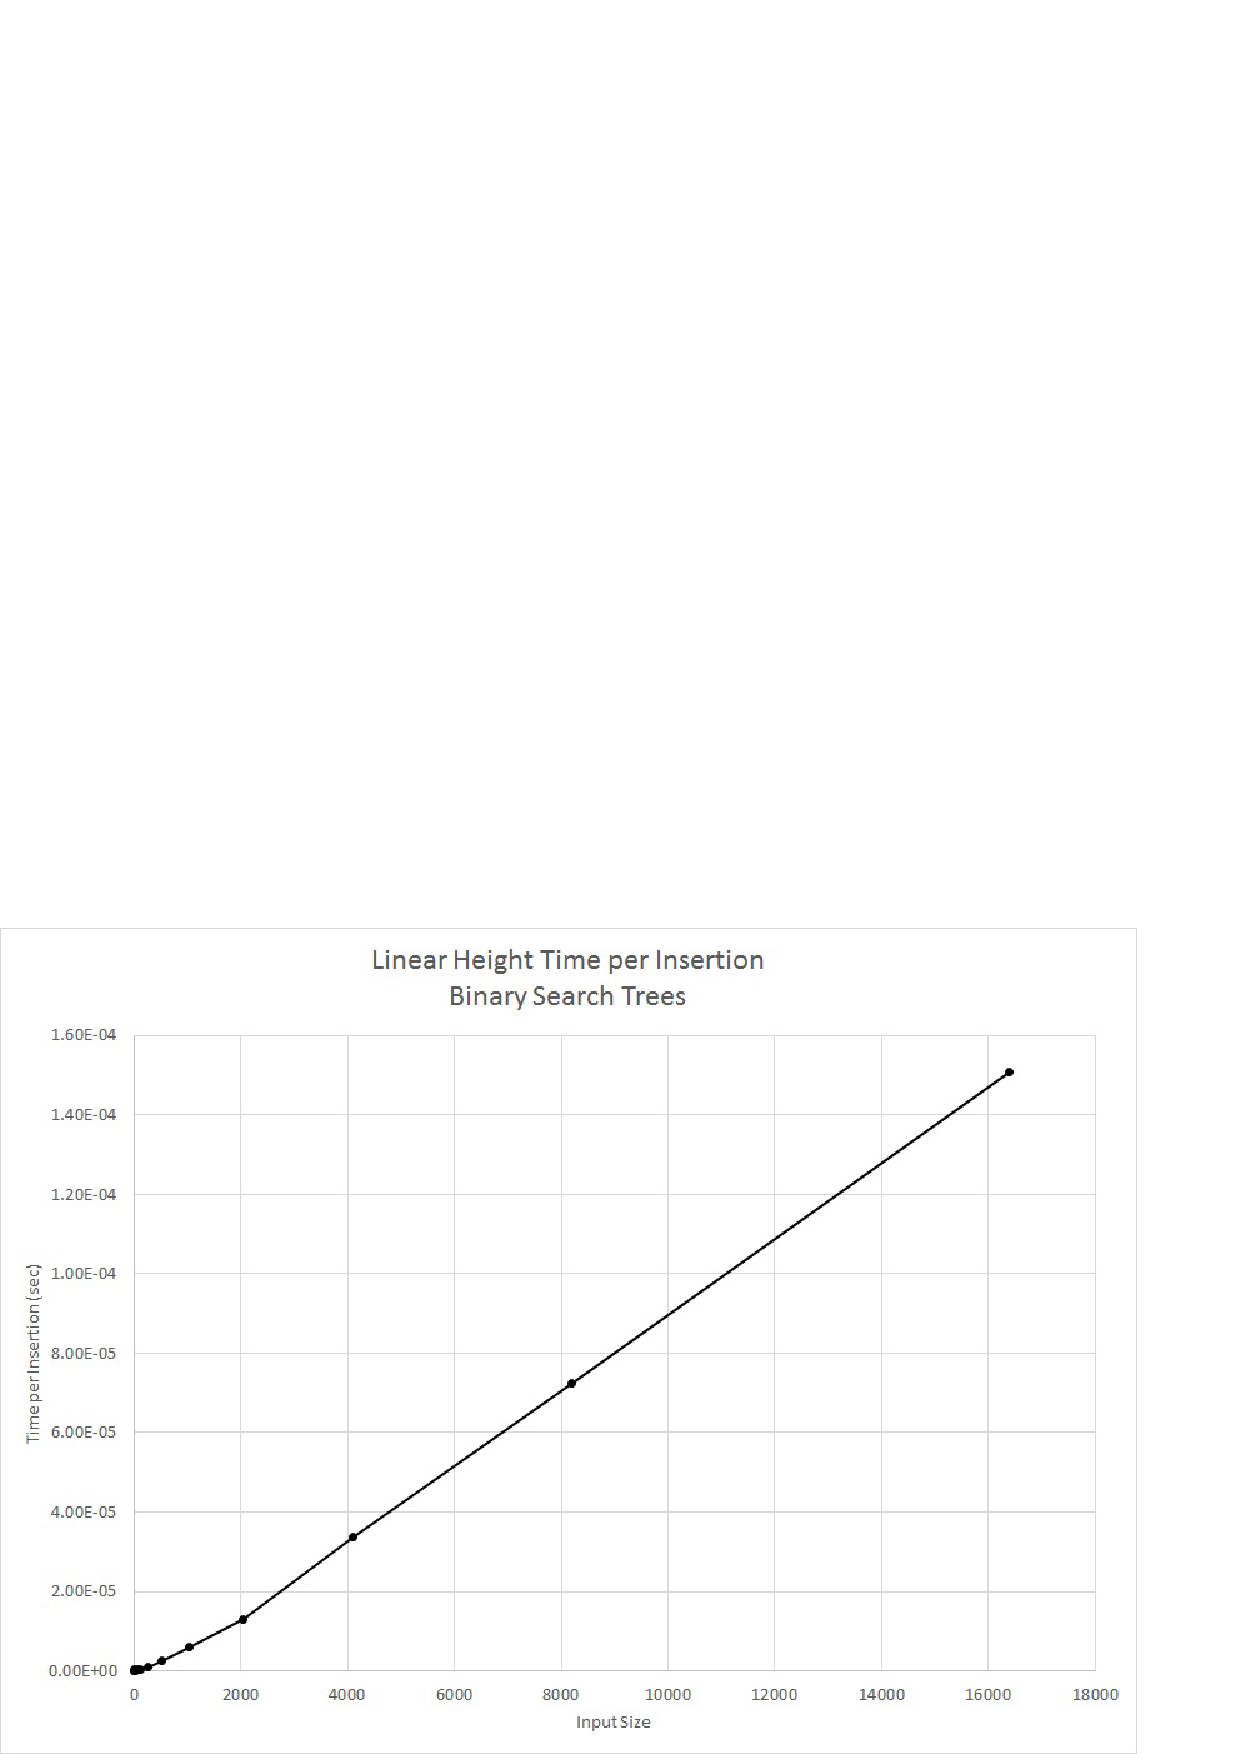
\includegraphics[width=11cm]{report/Linear_Time_Per_(Binary).jpg} \caption{Graph of the Time Taken per Addition for Different Input Sizes for a Linear Order Added Binary Search Tree} 
\label{fig:Linear_Time_Per_Binary}
\end{figure}

\begin{figure}[h]
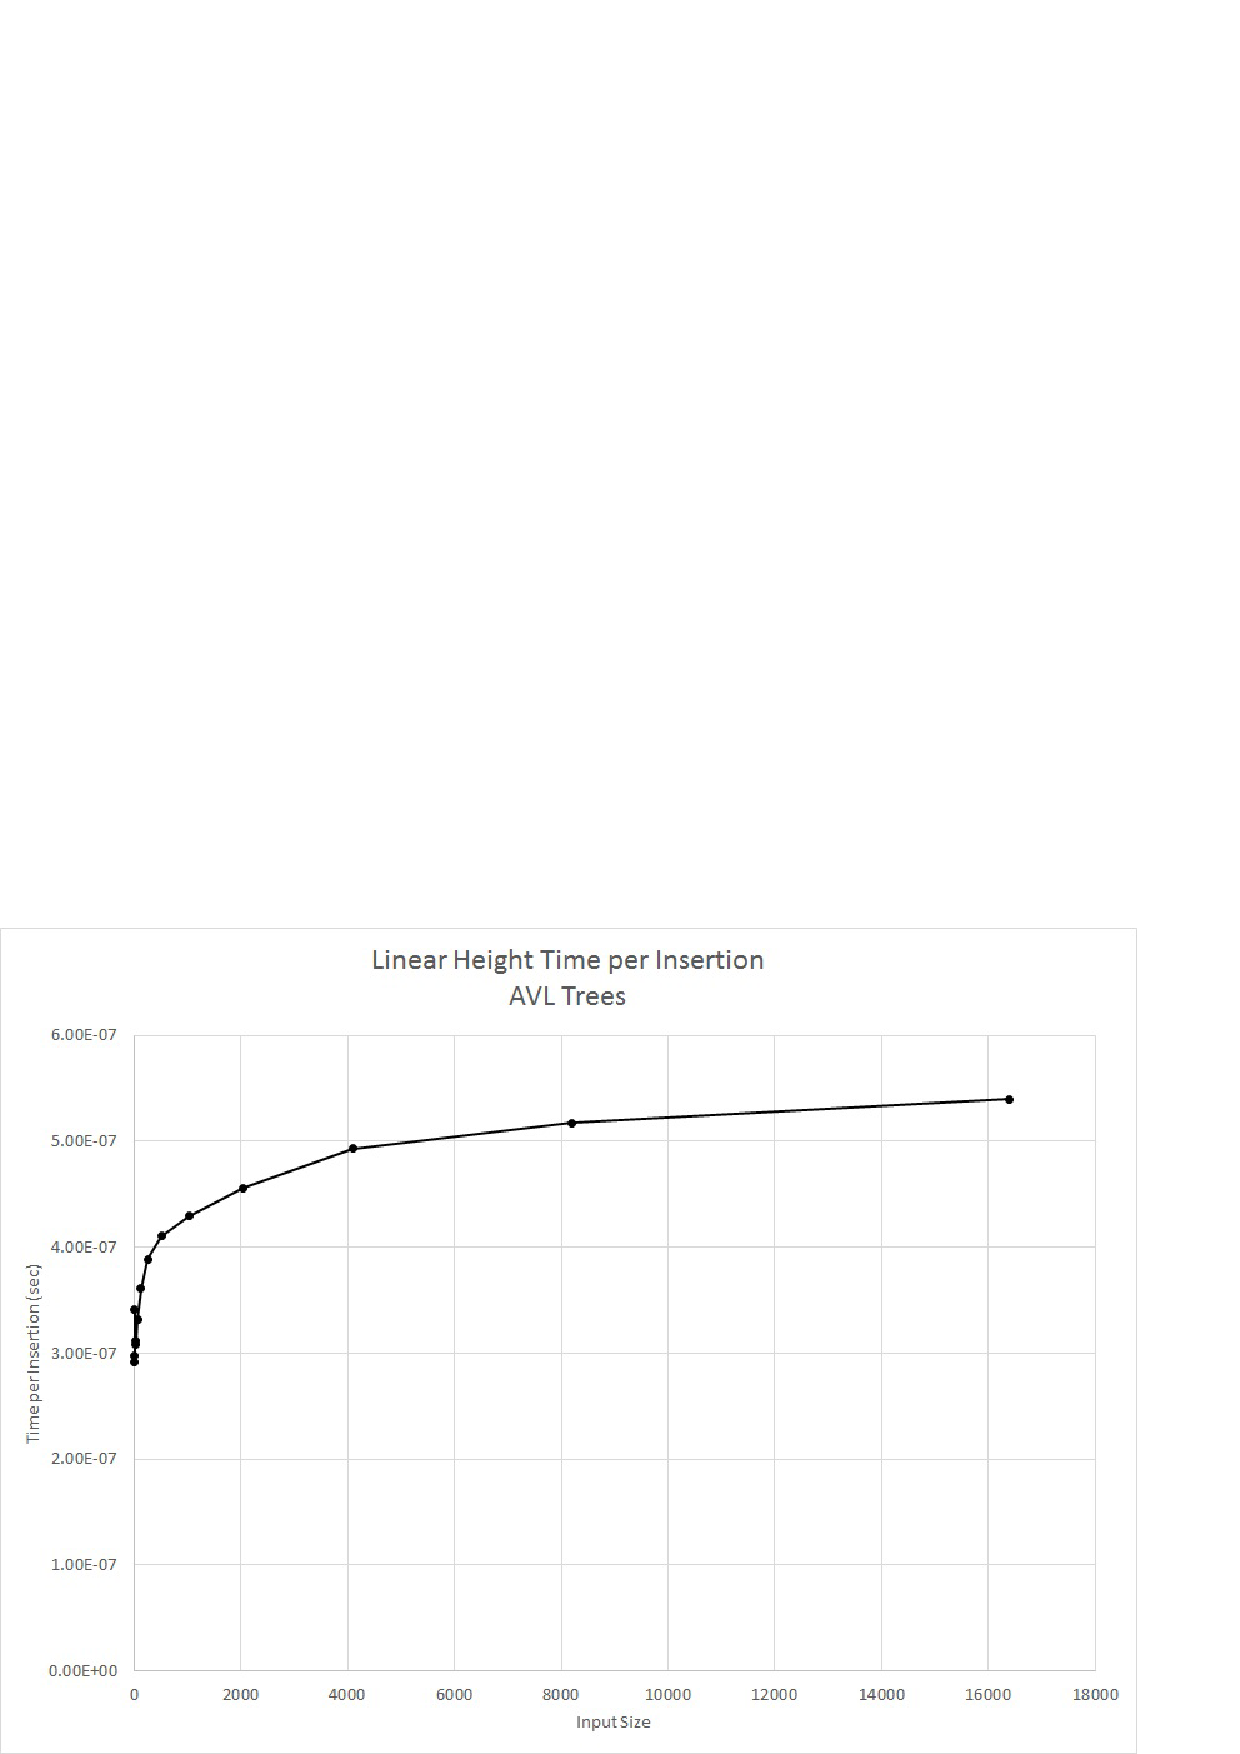
\includegraphics[width=11cm]{report/Linear_Time_Per_(AVL).jpg} \caption{Graph of the Time Taken for Different Input Sizes for a  Linear Order Added AVL Tree} 
\label{fig:Linear_Time_Per_AVL}
\end{figure}

\begin{figure}[h]
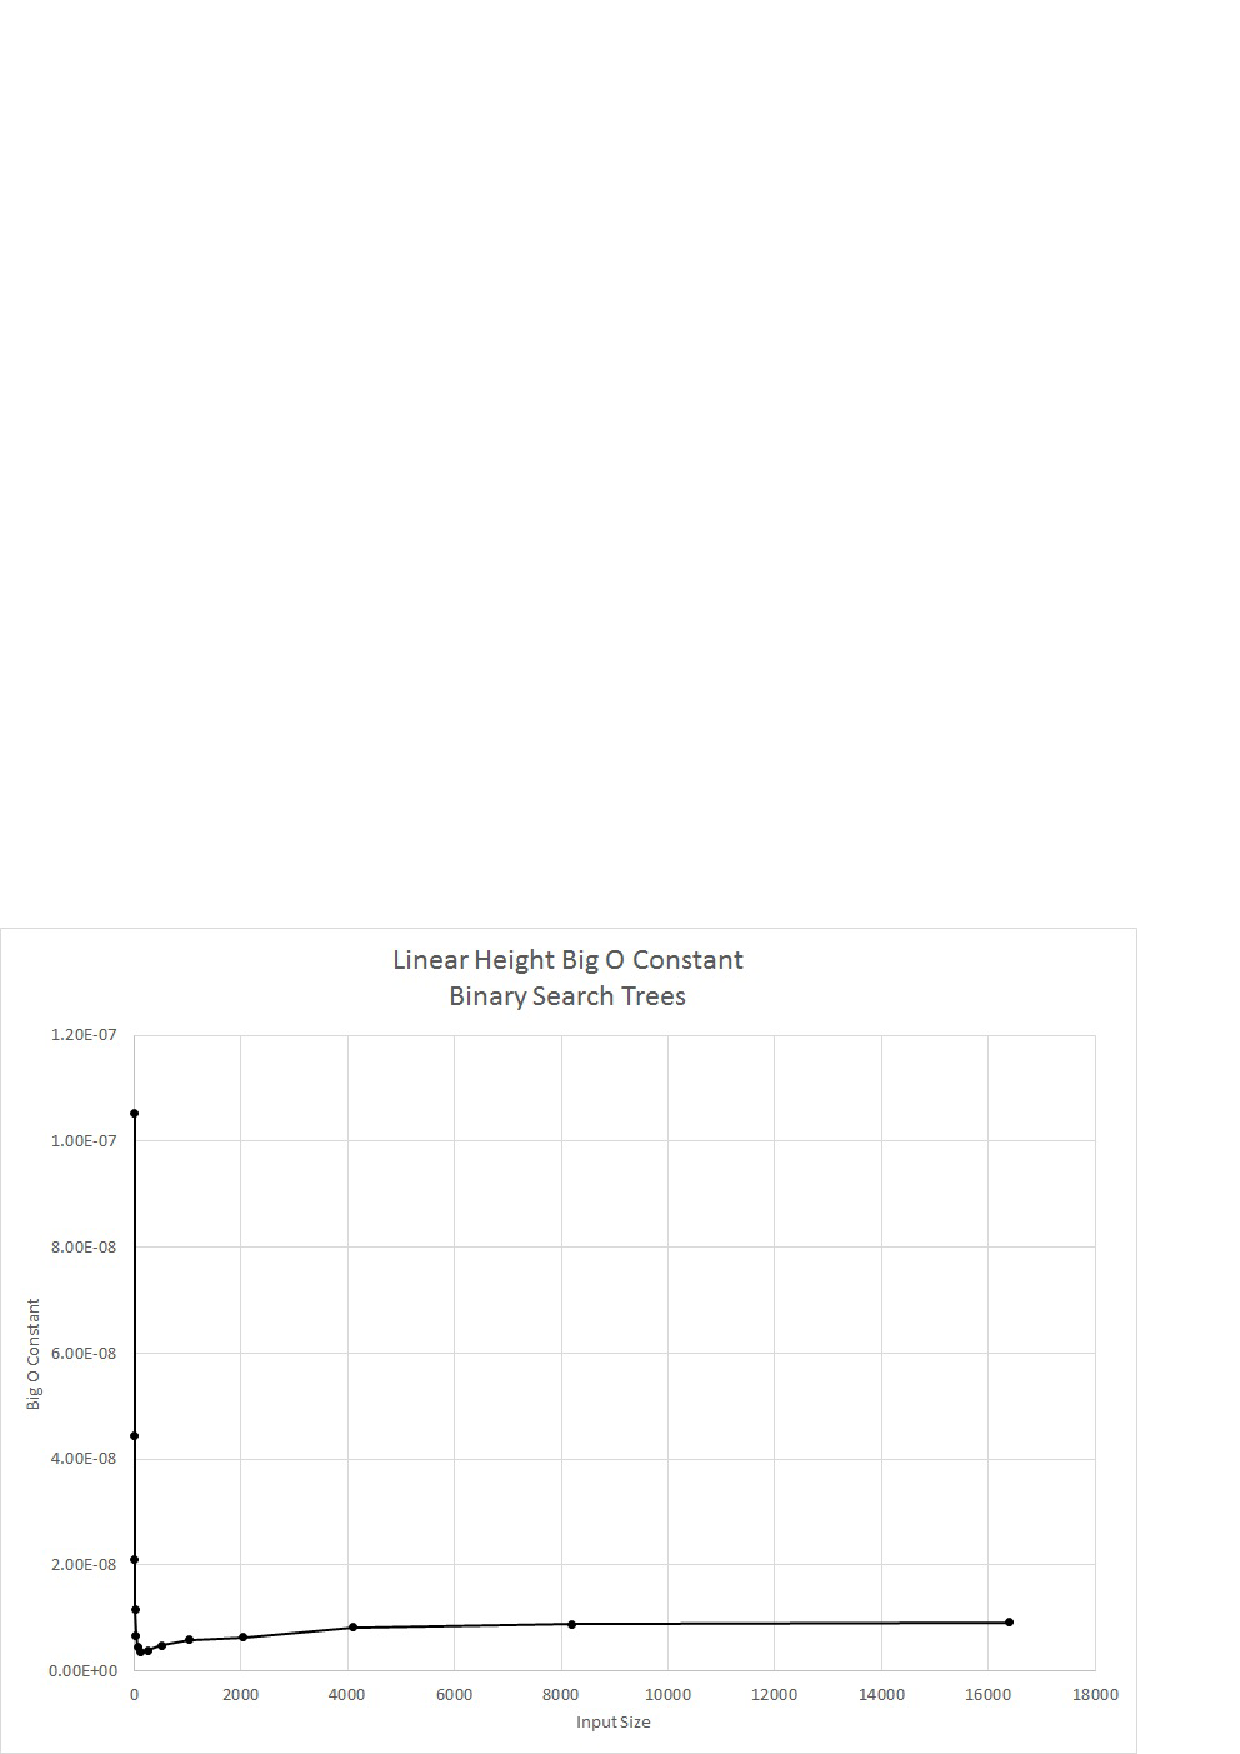
\includegraphics[width=11cm]{report/Linear_Big_O_(Binary).jpg} \caption{Graph of the Big O Constants for Different Input Sizes for a  Linear Order Added Binary Search Tree} 
\label{fig:Linear_Big_O_Binary}
\end{figure}

\begin{figure}[h]
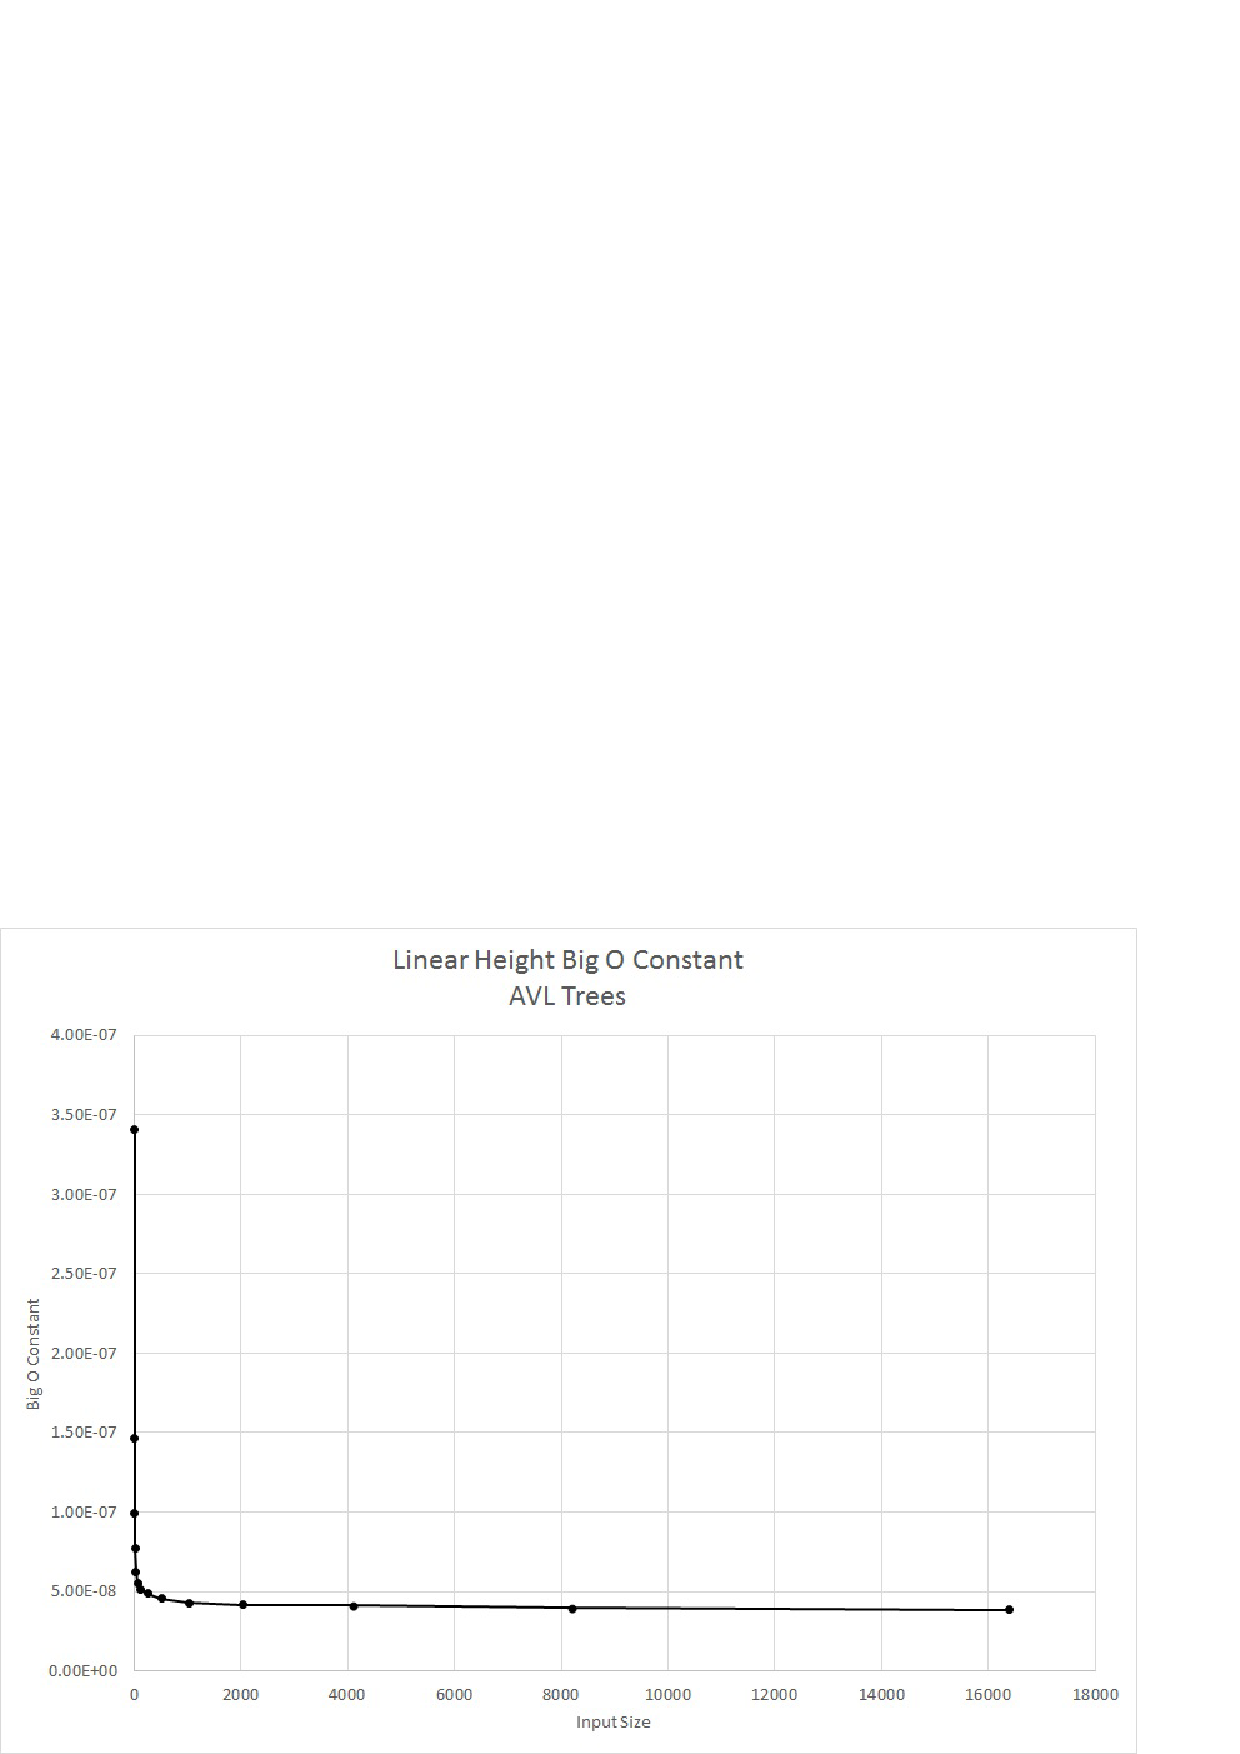
\includegraphics[width=11cm]{report/Linear_Big_O_(AVL).jpg} \caption{Graph of the Big O Constants for Different Input Sizes for a  Linear Order Added AVL Tree} 
\label{fig:Linear_Big_O_AVL}
\end{figure}

\begin{figure}[h]
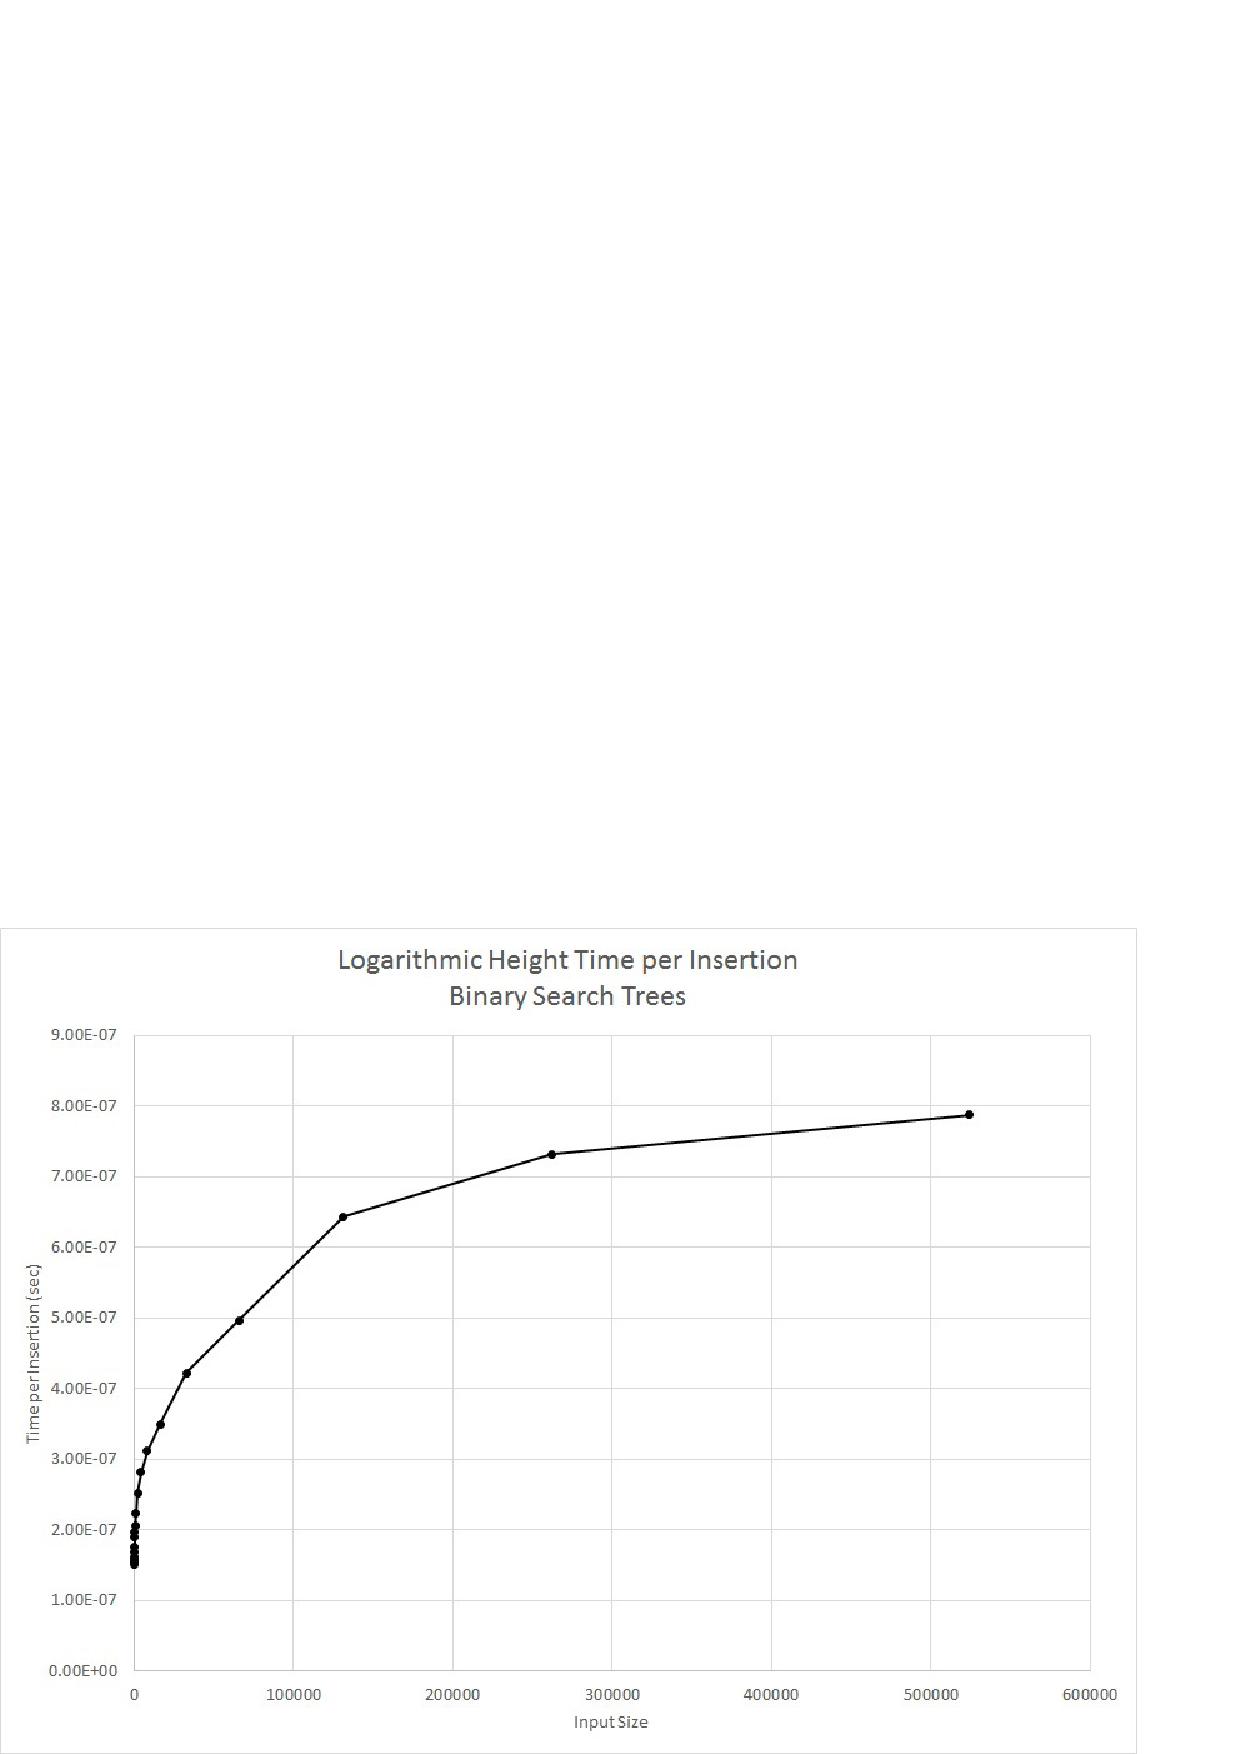
\includegraphics[width=11cm]{report/Logarithmic_Time_Per_(Binary).jpg} \caption{Graph of the Time Taken per Addition for Different Input Sizes for a Logarithmic Order Added Binary Search Tree} 
\label{fig:Logarithmic_Time_Per_Binary}
\end{figure}

\begin{figure}[h]
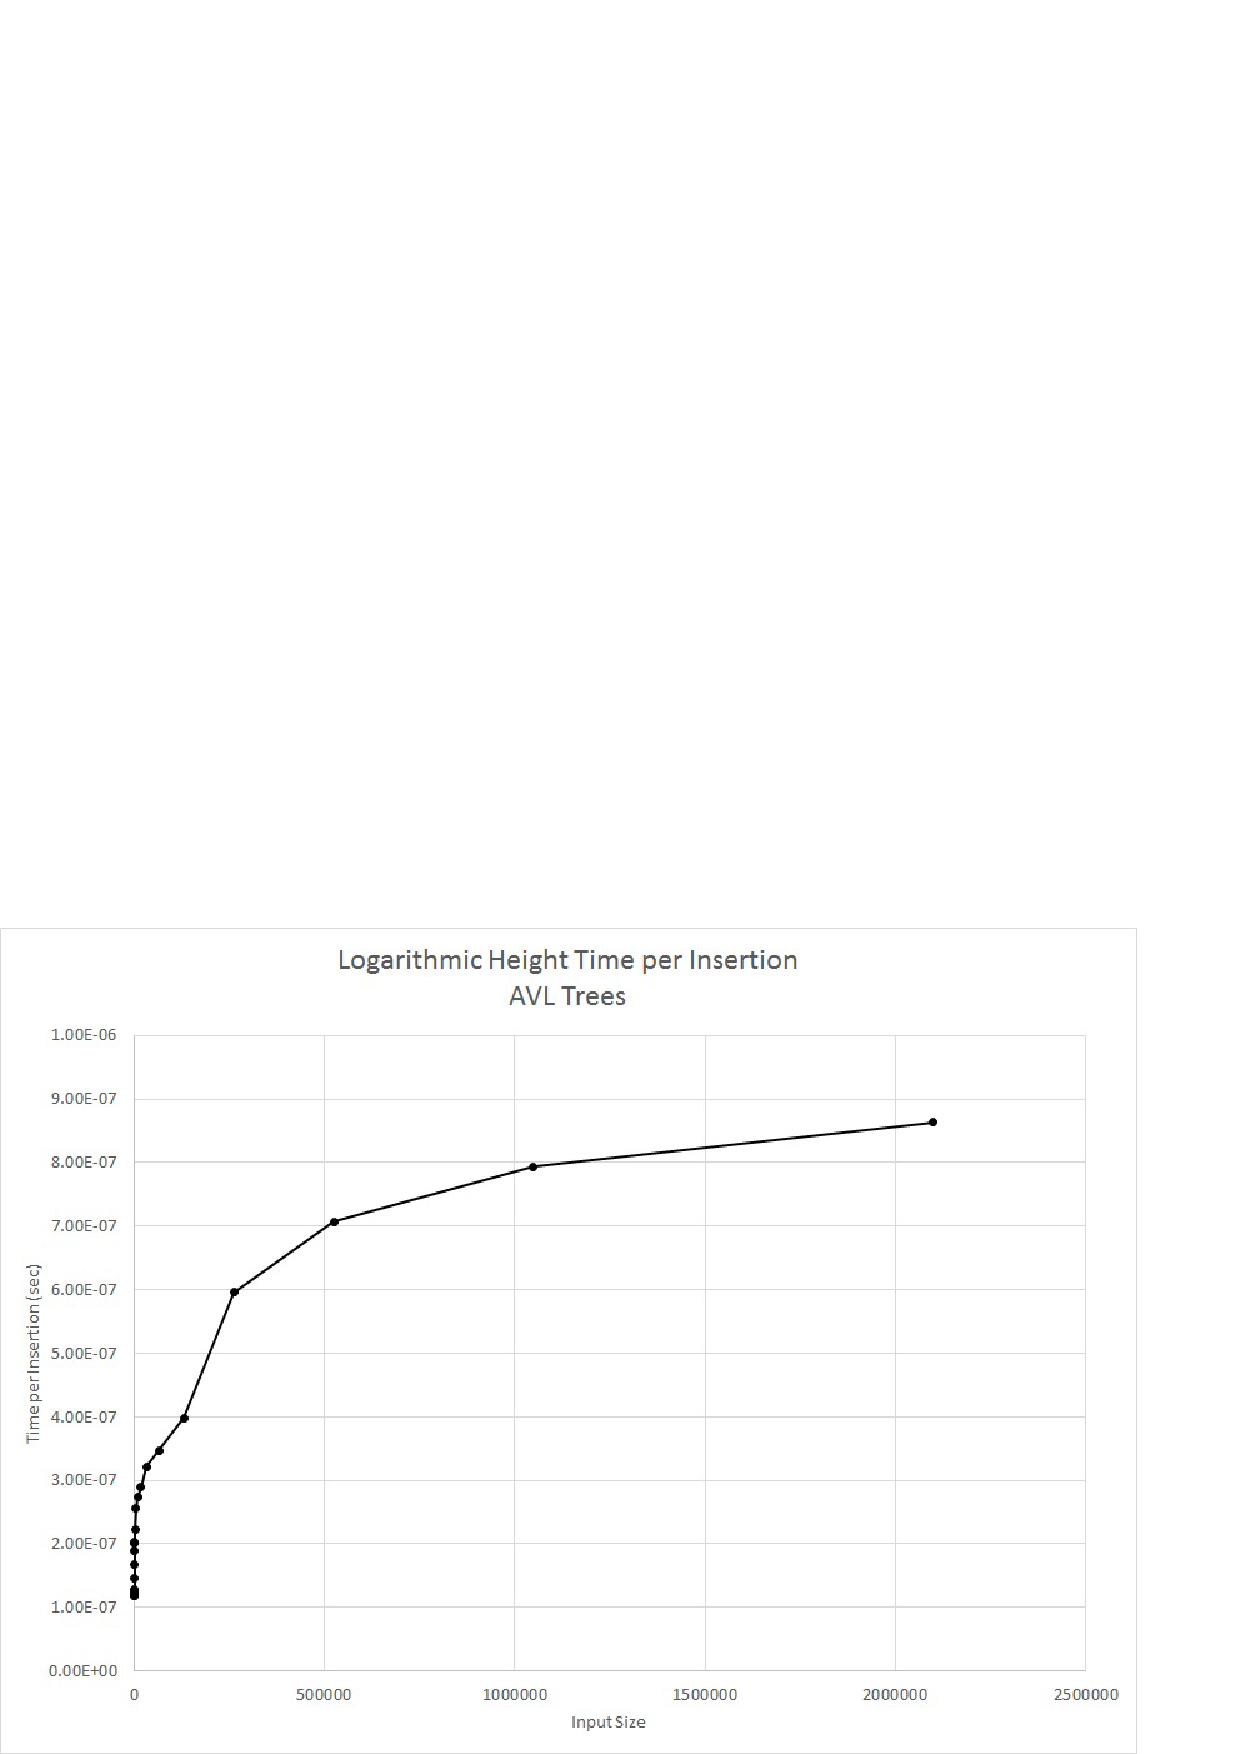
\includegraphics[width=11cm]{report/Logarithmic_Time_Per_(AVL).jpg} \caption{Graph of the Time Taken for Different Input Sizes for a  Logarithmic Order Added AVL Tree} 
\label{fig:Logarithmic_Time_Per_AVL}
\end{figure}

\begin{figure}[h]
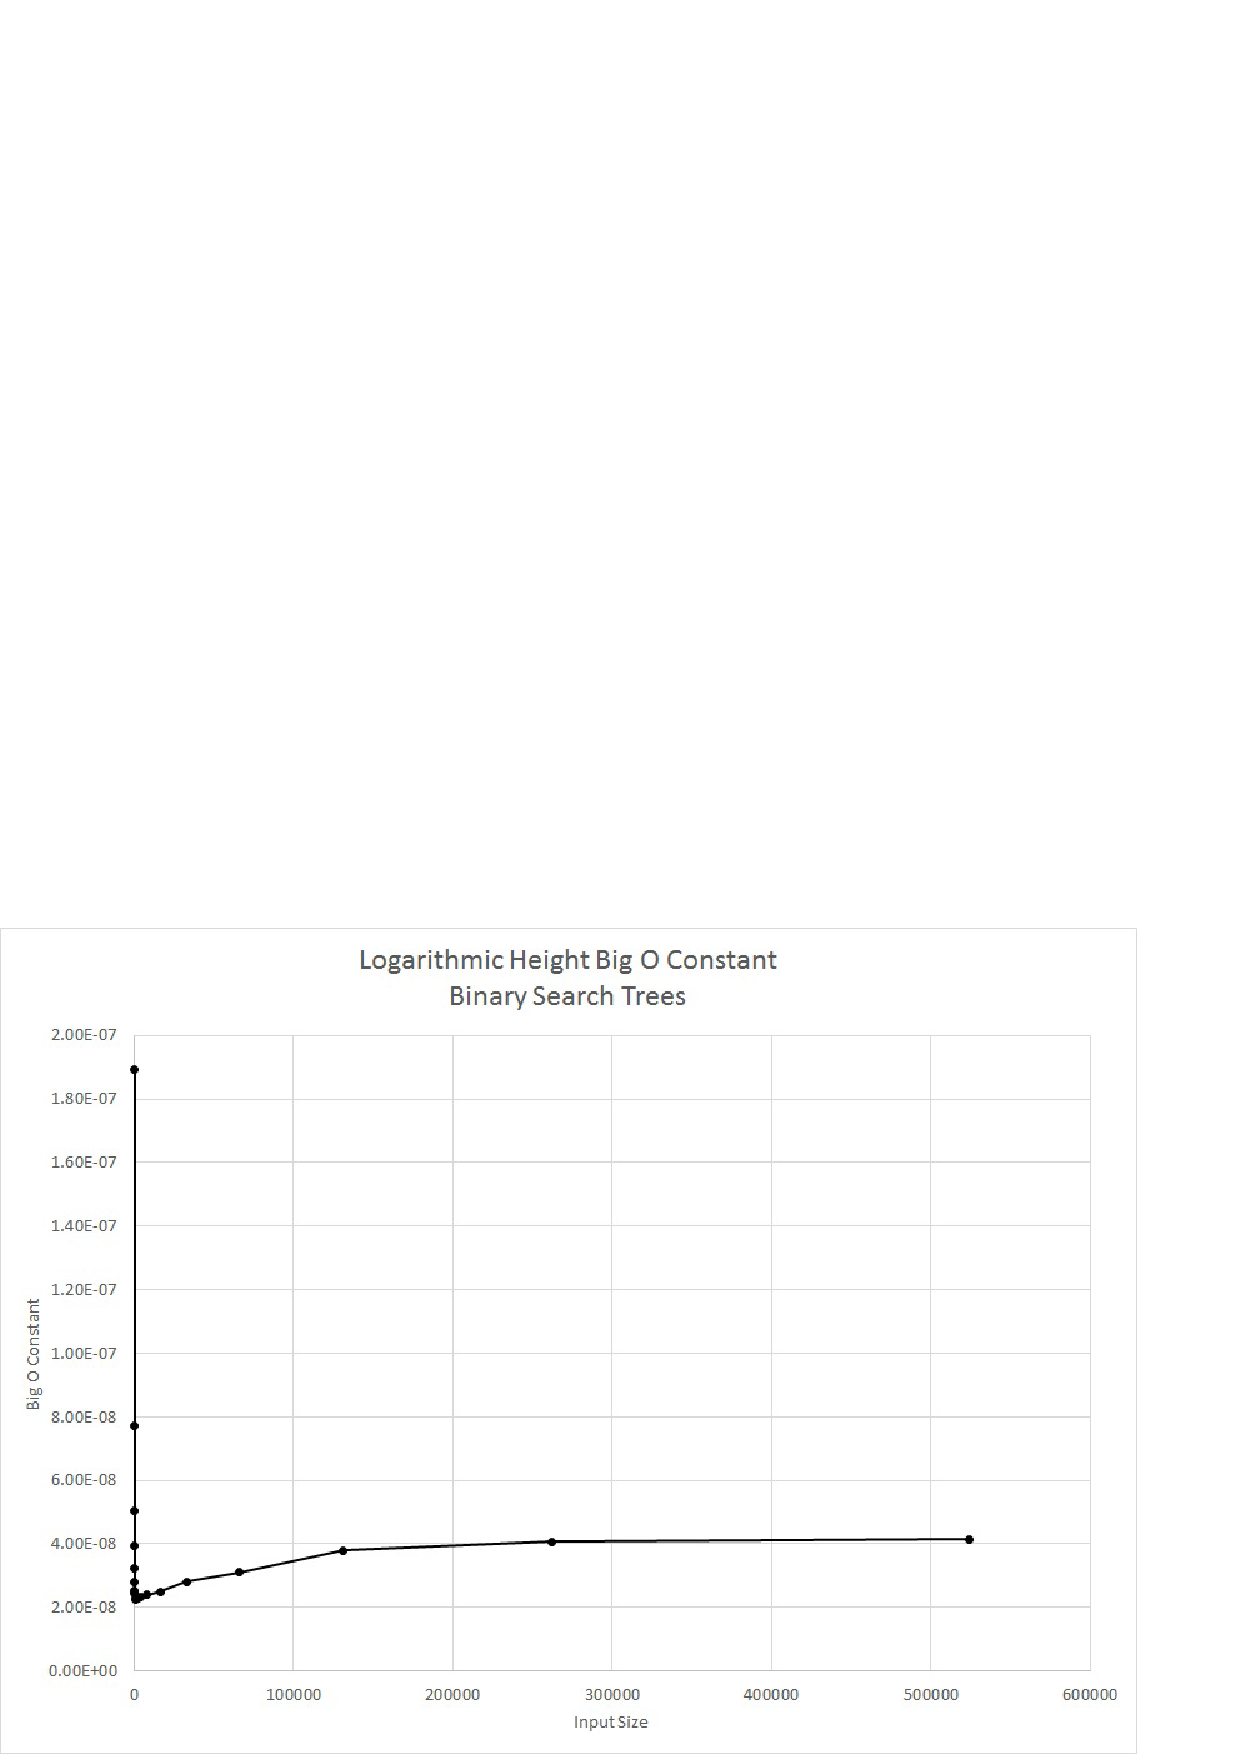
\includegraphics[width=11cm]{report/Logarithmic_Big_O_(Binary).jpg} \caption{Graph of the Big O Constants for Different Input Sizes for a  Logarithmic Order Added Binary Search Tree} 
\label{fig:Logarithmic_Big_O_Binary}
\end{figure}

\begin{figure}[h]
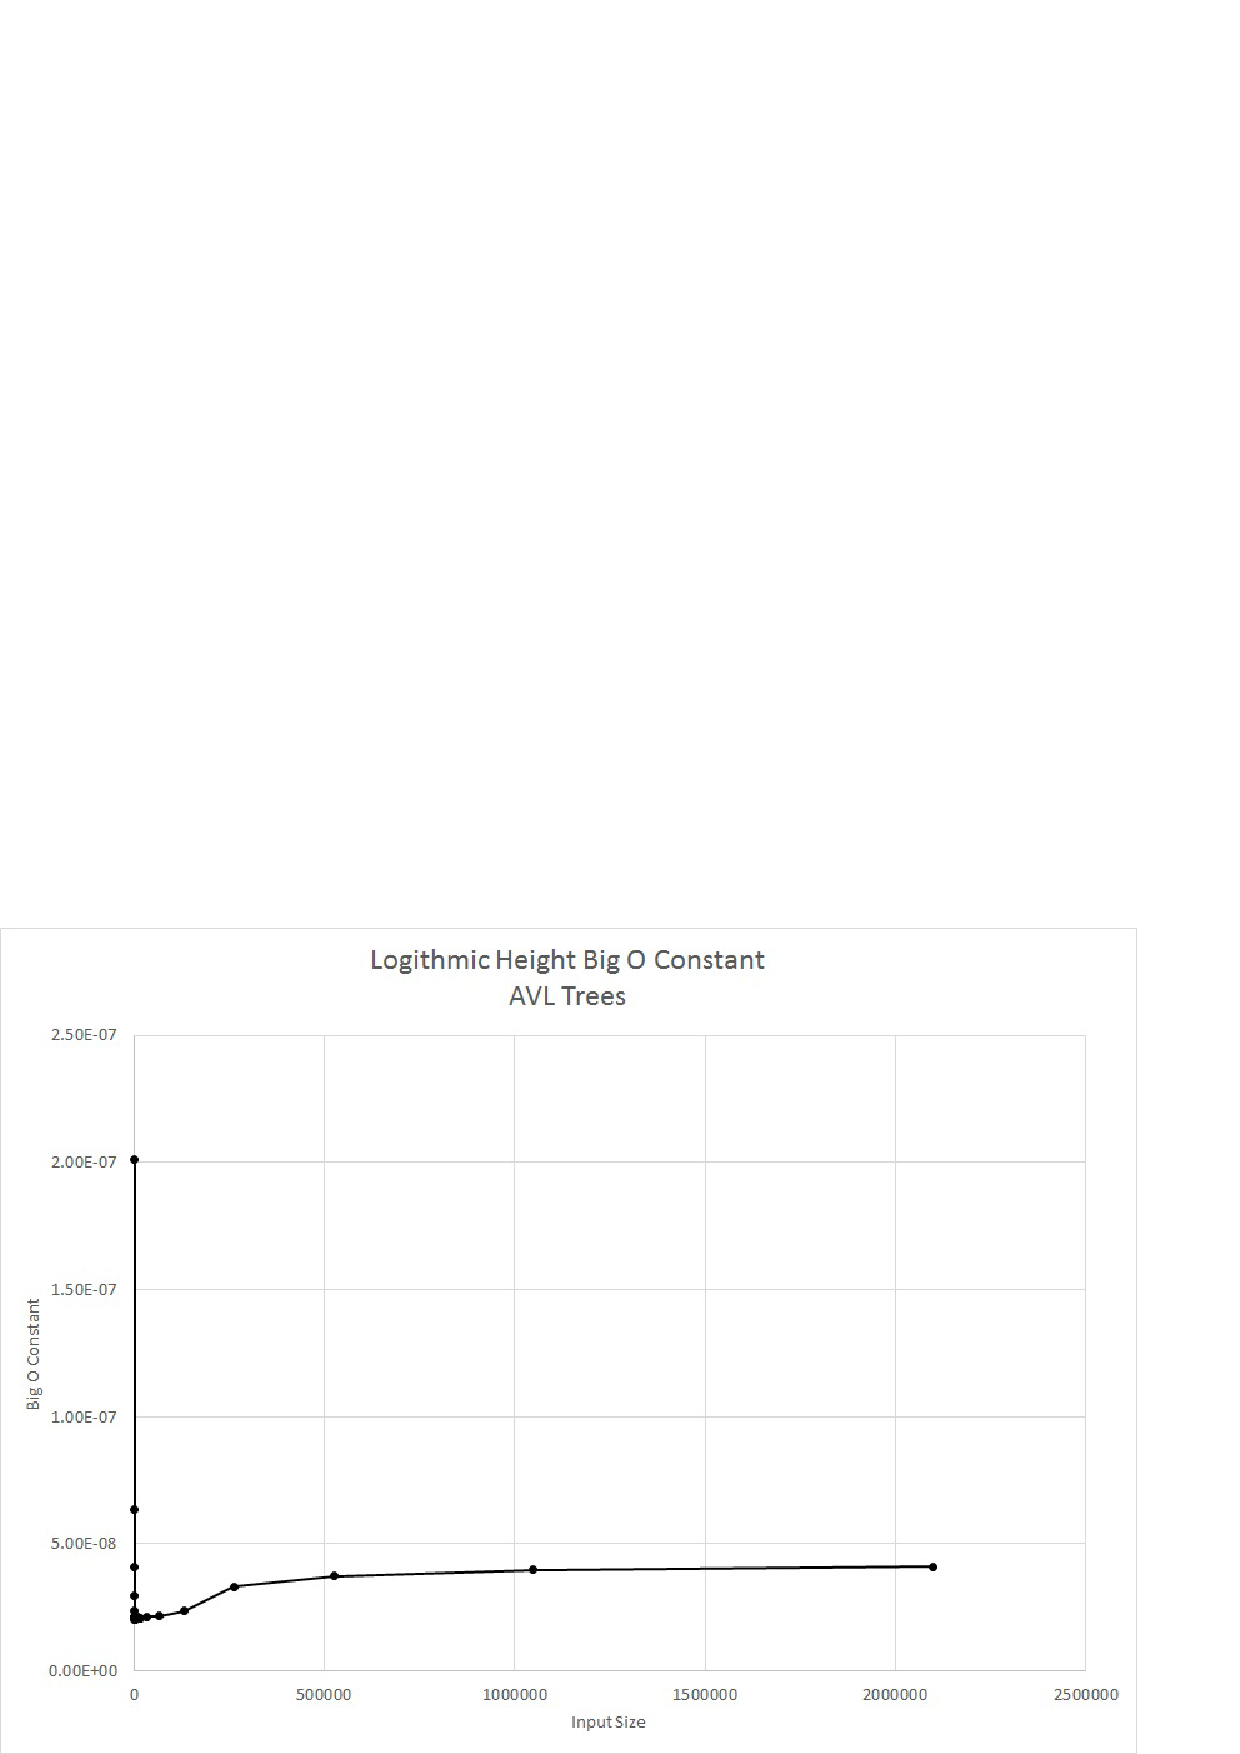
\includegraphics[width=11cm]{report/Logarithmic_Big_O_(AVL).jpg} \caption{Graph of the Big O Constants for Different Input Sizes for a  Logarithmic Order Added AVL Tree} 
\label{fig:Logarithmic_Big_O_AVL}
\end{figure}

\begin{figure}[h]
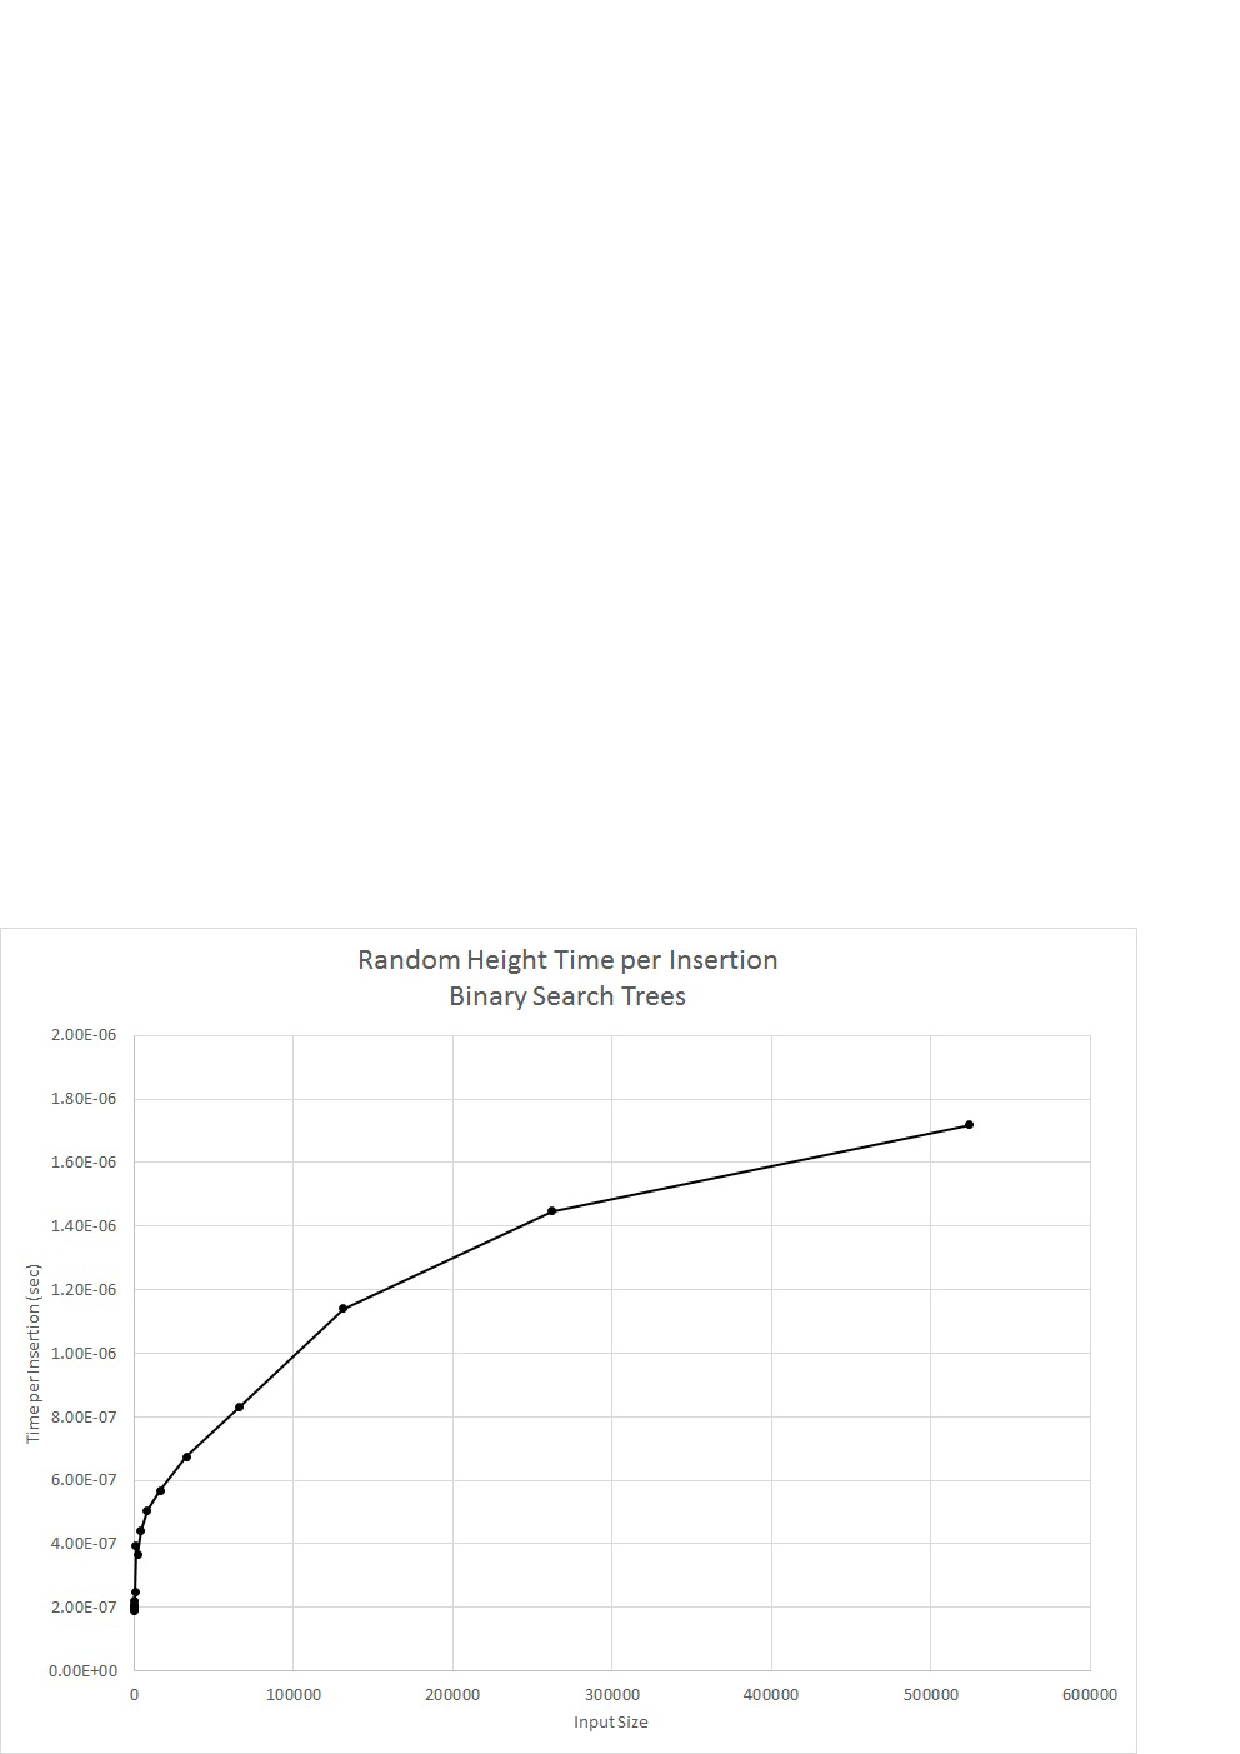
\includegraphics[width=11cm]{report/Random_Time_Per_(Binary).jpg} \caption{Graph of the Time Taken per Addition for Different Input Sizes for a Random Order Added Binary Search Tree} 
\label{fig:Random_Time_Per_Binary}
\end{figure}

\begin{figure}[h]
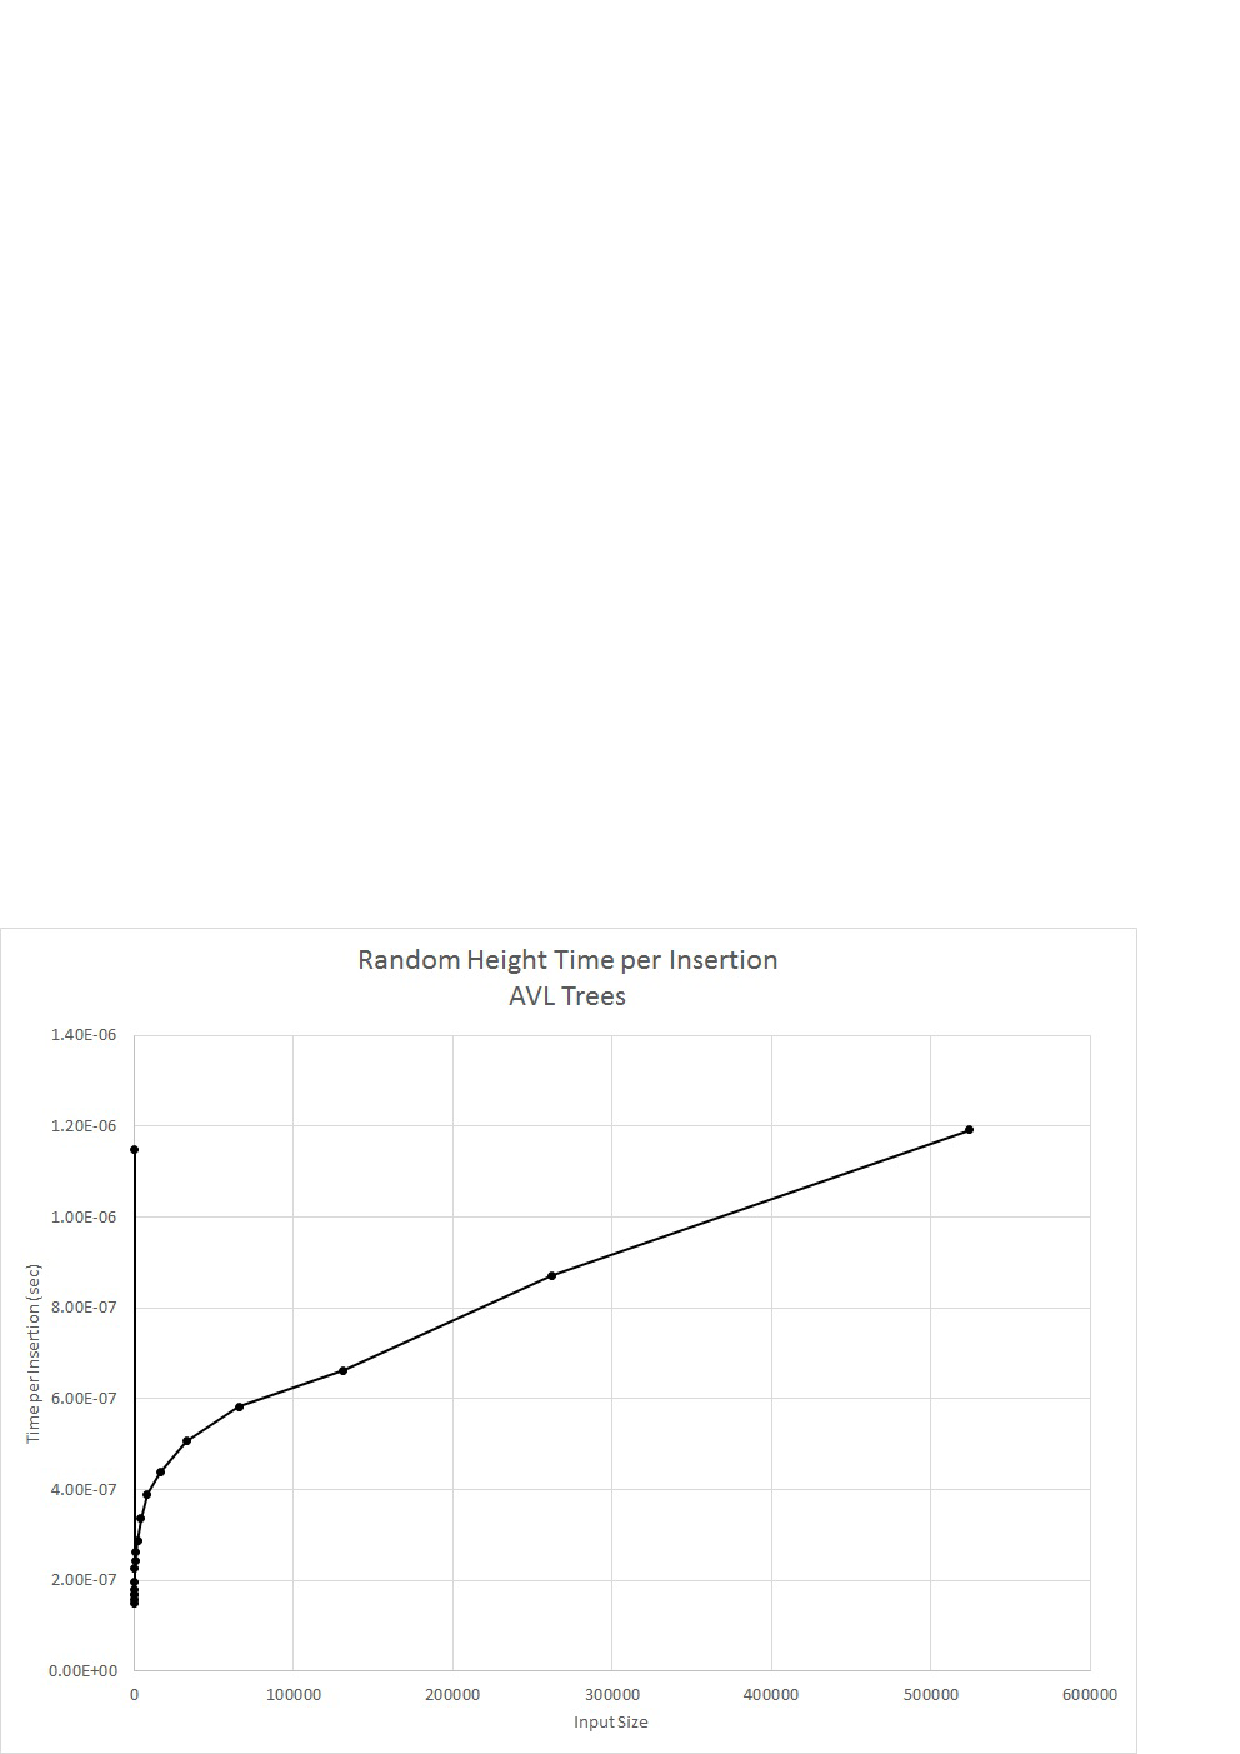
\includegraphics[width=11cm]{report/Random_Time_Per_(AVL).jpg} \caption{Graph of the Time Taken for Different Input Sizes for a  Random Order Added AVL Tree} 
\label{fig:Random_Time_Per_AVL}
\end{figure}

\begin{figure}[h]
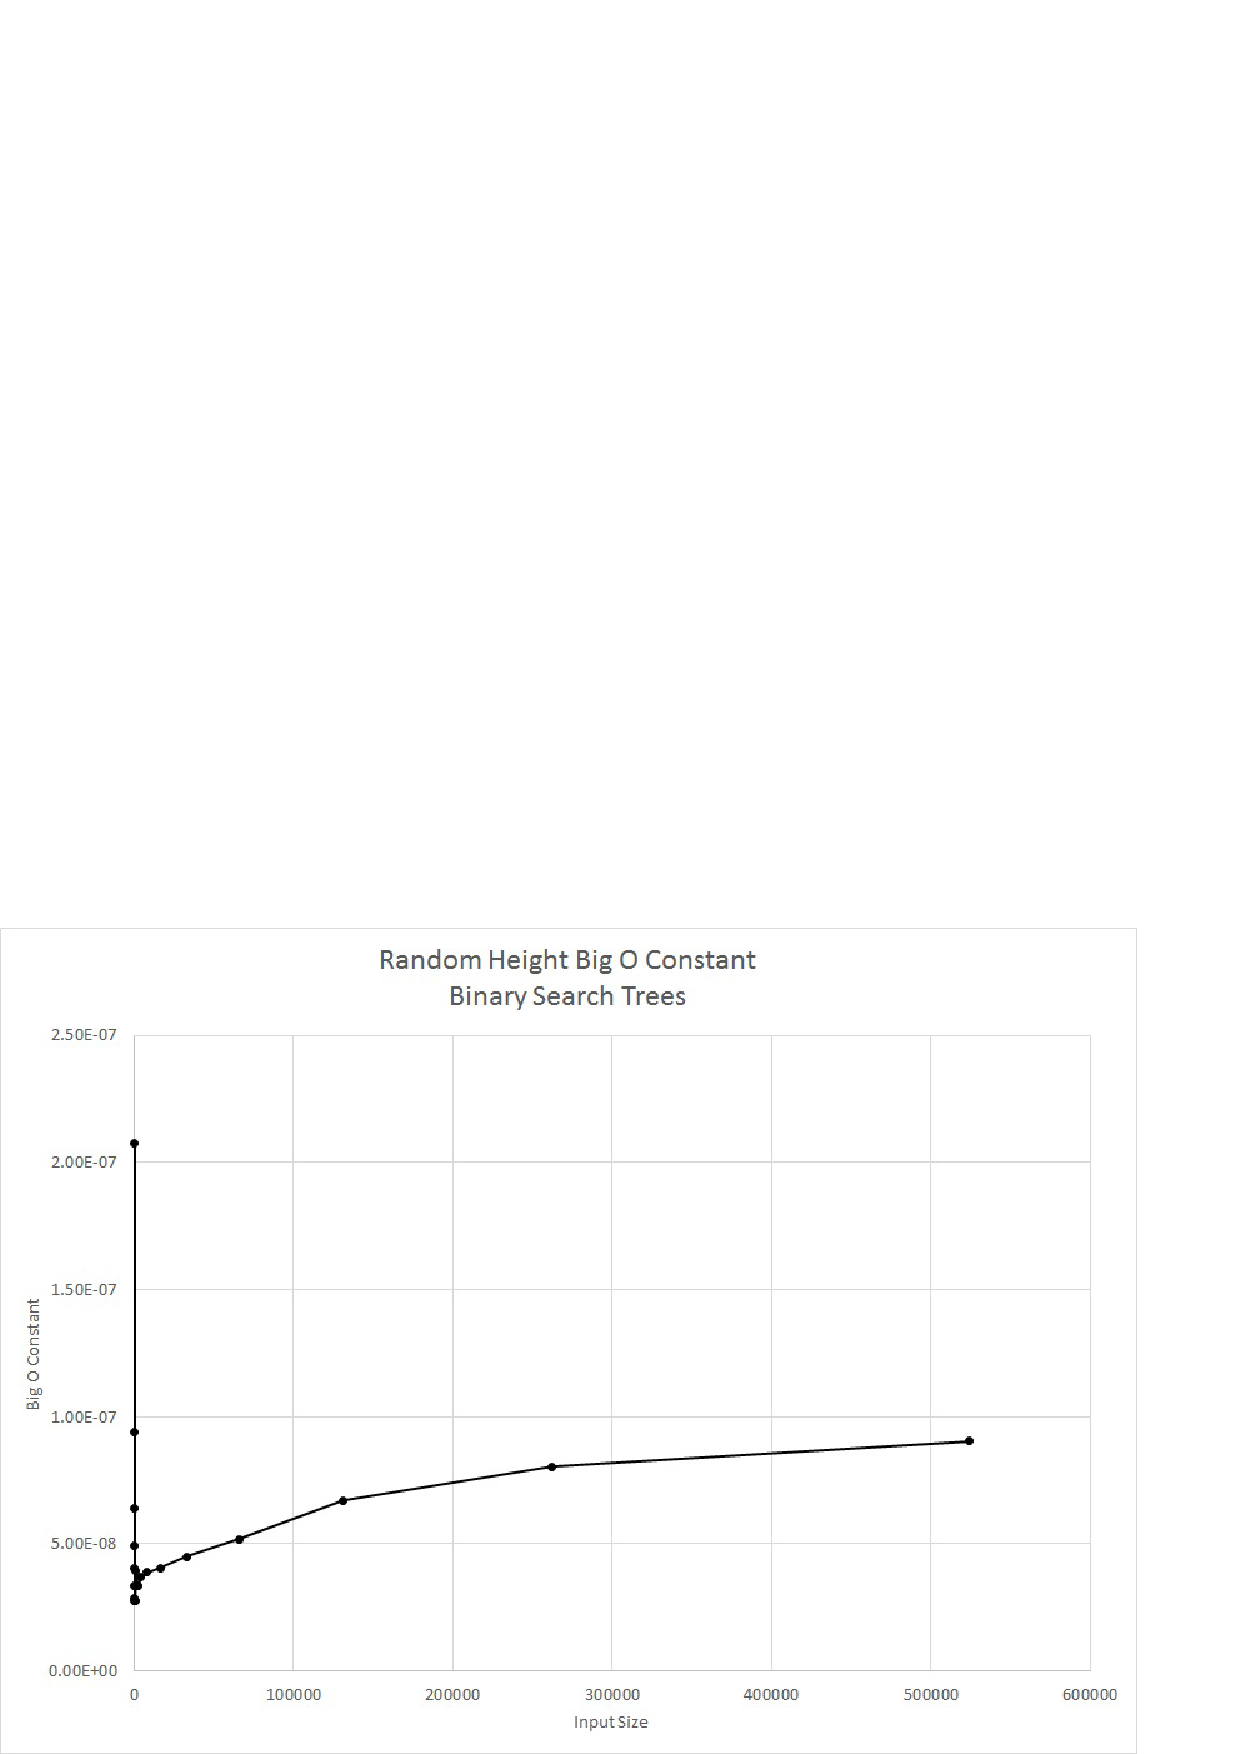
\includegraphics[width=11cm]{report/Random_Big_O_(Binary).jpg} \caption{Graph of the Big O Constants for Different Input Sizes for a  Random Order Added Binary Search Tree} 
\label{fig:Random_Big_O_Binary}
\end{figure}

\begin{figure}[h]
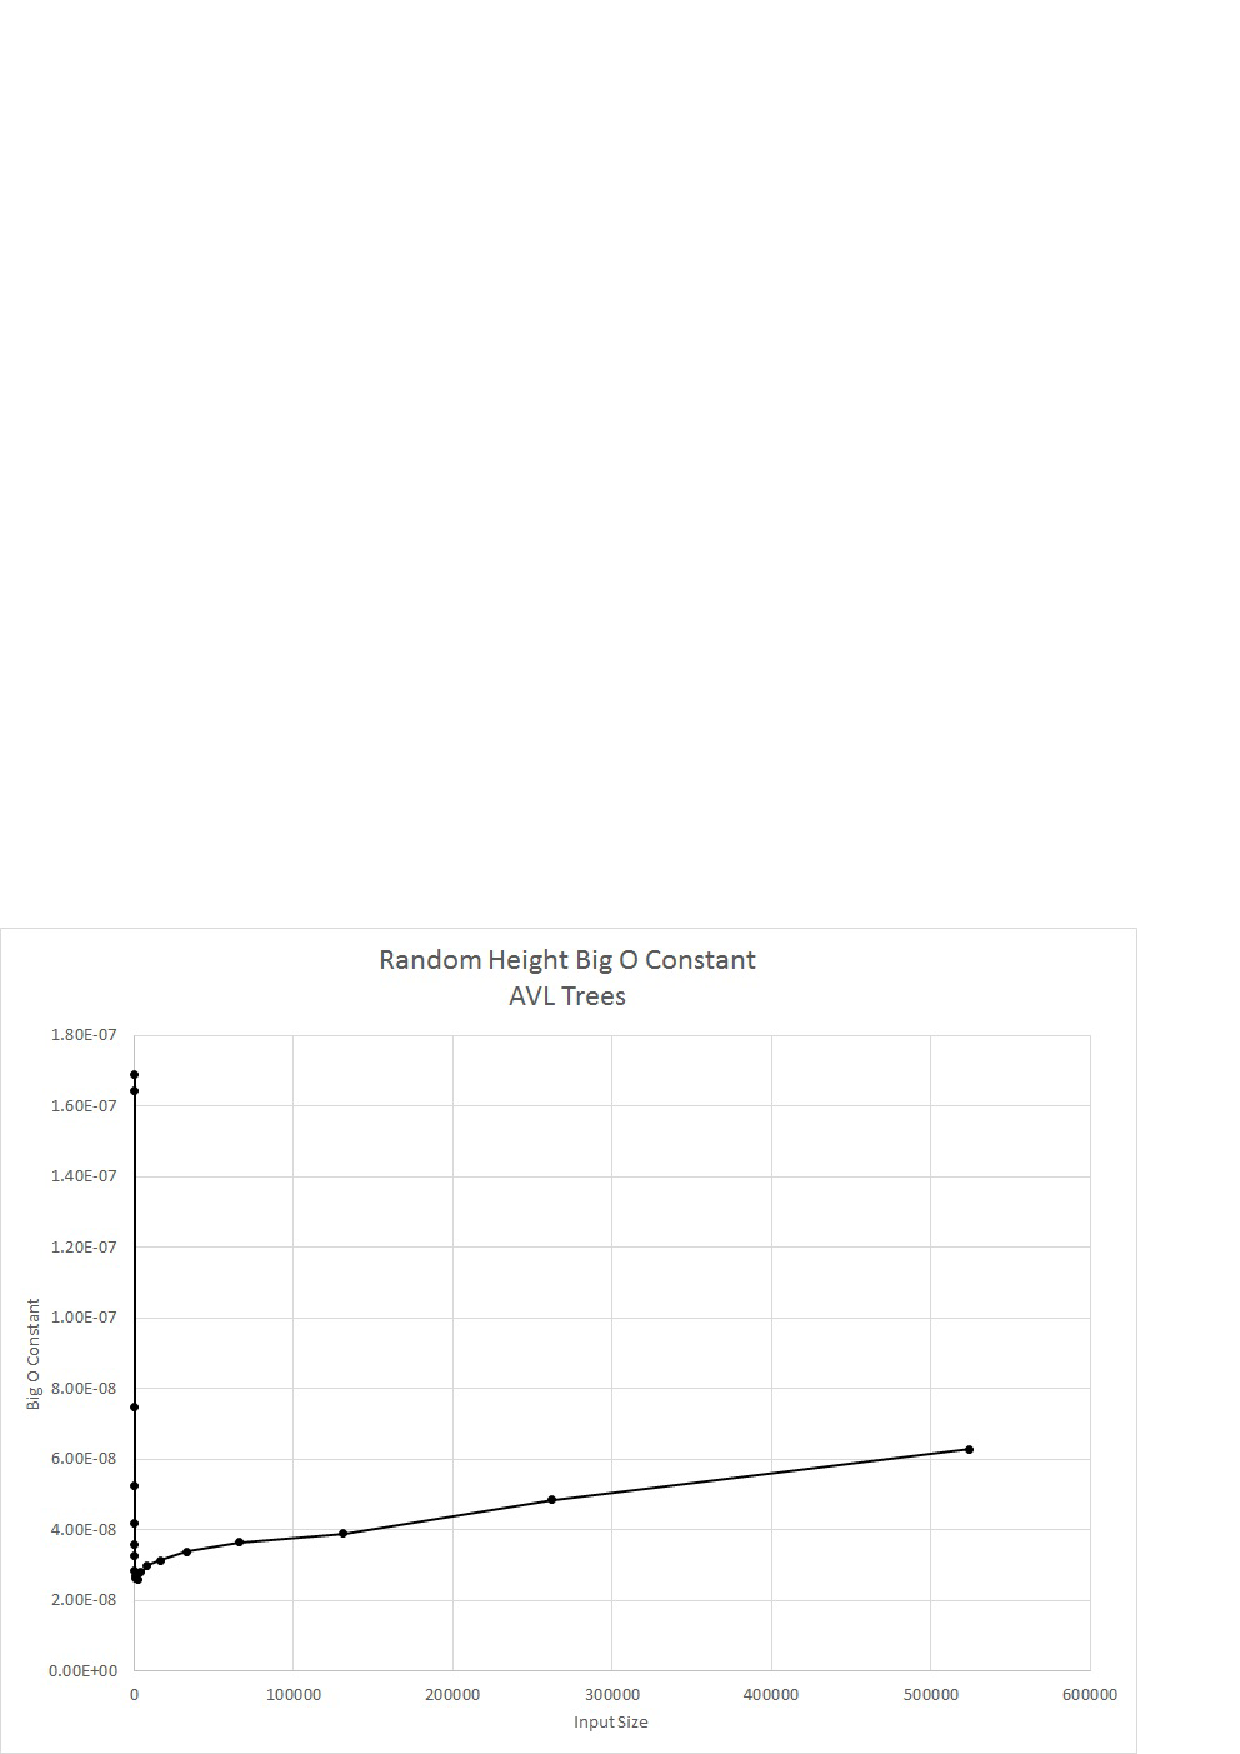
\includegraphics[width=11cm]{report/Random_Big_O_(AVL).jpg} \caption{Graph of the Big O Constants for Different Input Sizes for a  Random Order Added AVL Tree} 
\label{fig:Random_Big_O_AVL}
\end{figure}

\section*{Conclusion}
\end{document}
